 \documentclass[color={usenames, dvipsnames},ignorenonframetext]{beamer}
% \documentclass{article}
% \usepackage{beamerarticle}
\usepackage{fancyvrb}
\usepackage{amsmath}
\usepackage{amsfonts}
\usepackage{multirow}
\usepackage{booktabs}

\newcommand{\A}{\mathbf{A}}
\newcommand{\DA}{\mathbf{\Delta A}}
\newcommand{\qp}{q^{(+)}(x)}
\newcommand{\qm}{q^{(-)}(x)}

\renewcommand\multirowsetup{\centering}
\newlength\LL \settowidth\LL{100}

\mode<article>{\usepackage{fullpage}}
\mode<presentation>{\usetheme{AnnArbor}}
%\mode<presentation>{\usecolortheme{wolverine}}

\setbeamertemplate{navigation symbols}{}    % Remove navigation symbols

\author[JLC]{Jeremy Lloyd Conlin \\ \texttt{jlconlin@umich.edu}}

\institute[UM]{University of Michigan, Ann Arbor, Michigan}

\title[Monte Carlo Arnoldi]{Arnoldi's Method for Monte Carlo Criticality Calculations}

\date[ORNL]{Oak Ridge National Laboratory}

\begin{document}
\begin{abstract}
    The power method has been the algorithm of choice for Monte Carlo criticality codes for decades.  The power method can only calculate the fundamental eigenmode and suffers from slow convergence.  Despite its limitations, Monte Carlo codes have continued to use it because it is simple to implement and is consistent.

    Arnoldi's method of minimized iterations has been used in the computer science field for many years to calculate the eignvalues and eigenvectors of a matrix.  It is particularly interesting for sparse matrices or matrix-free applications where an explicit form of the matrix is not known.  

    Arnoldi's method has a great advantage over the power method as it can calculate multiple eigenmodes.  Recent work has also shown the possibility of reducing the computational expense of calculating the matrix-vector product by reducing the precision of matrix-vector product.  This can be done without altering the convergence of the calculation.  

    My PhD research has focused on using Arnoldi's method in a Monte Carlo criticality application.  I have implemented Arnoldi's method in a slab-geometry Monte Carlo code and have compared it to the power method.  In my talk I will present what I have learned about Arnoldi's method.  I will show comparisons between Arnoldi's method and the power method for slab geometry problems.  I will also discuss some work that remains to be done.
\end{abstract}

\begin{frame} 
    \titlepage 
\end{frame}

\begin{frame}
    \frametitle{Outline}
    \tableofcontents[pausesection]
\end{frame}

\section{Krylov Subspace Methods}
\begin{frame}
    \frametitle{Krylov Subspace Methods}
    Krylov Subspace:
    \begin{equation*}
        \mathcal{K}_m~=~\mathrm{span}\left\{v, \A v, \A^2v, \ldots , \A^{m-1}v\right\}
    \end{equation*}
    \begin{itemize}
        \item Constructed iteratively
            \note{We could construct the subspace the inefficient way by taking the power of the linear operator multiple times then operate on the vector.  Or we can just  operate on the previously calculated Krylov vector.}
        \item Don't require explicit knowledge of linear operator
        \item Perfect for Monte Carlo criticality applications
    \end{itemize}
\end{frame}

\begin{frame}
    \frametitle{Particle Transport Equation}
    \begin{itemize}
        \item Boltzmann Equation:
        \begin{equation*}
            \mathbf{\Omega}\cdot\mathbf{\nabla}\psi(\mathbf{r},\mathbf{\Omega})+\Sigma_t\psi(\mathbf{r},\mathbf{\Omega}) - \frac{\Sigma_s}{4\pi}\int \psi(\mathbf{r},\mathbf{\Omega})\;d\Omega =  \frac{1}{k}\frac{\nu\Sigma_f}{4\pi}\int \psi(\mathbf{r},\mathbf{\Omega})\;d\Omega
        \end{equation*}
        \item Operator Form:
        \begin{align*}
            \left(\mathbf{L} + \mathbf{C} - \mathbf{S}\right)\psi &= \frac{1}{k}\mathbf{F}\psi \\
            \mathbf{T}\psi &= \frac{1}{k}\mathbf{F}\psi
        \end{align*}
        \item Define:
        \begin{equation*}
            q \equiv \mathbf{F}\psi \hspace{5em} \A \equiv\mathbf{FT}^{-1}
        \end{equation*}
        \item Finally:
        \begin{equation*}
            \A q = kq
        \end{equation*}
    \end{itemize}
\end{frame}

\begin{frame}
    \frametitle{Monte Carlo Application of $\A$}
    \begin{align*}
        \A q &= kq \\
        q_{m+1} &= \frac{1}{k_m}\A q_m
    \end{align*}
    \begin{itemize}
        \item $q_m$ is a fission source
        \note{A fission source is a collection of fission sites}
        \item Neutron is sampled from $q_m$ and transported
        \item New fission sites are generated at points where neutron causes fission
    \end{itemize}
\end{frame}

\section{Power Method}
\begin{frame}
    \frametitle{Krylov Subspace---Power Method}
    \begin{equation*}
        \mathcal{K}_m~=~\mathrm{span}\left\{v, \A v, \A^2v, \ldots , \A^{m-1}v\right\}
    \end{equation*}
    \begin{itemize}
        \item Straightforward implementation of a Krylov Subspace
        \item Subspace becomes ``not-helpful'' because Krylov vectors are all nearly the same
    \end{itemize}
\end{frame}

\begin{frame}
    \frametitle{Krylov Subspace---Power Method}
    Power Iteration:
    \begin{gather*}
        q_{m+1} = \frac{1}{k_{m}}\mathbf{A}q_{m}, \\[2mm]
        k_{m+1} = k_{m}\frac{\int \A q_{m}}{\int q_{m}} = k_{m}\frac{\sum_{i=1}^{N} \omega_{m+1}^{(i)}}{\sum_{i=1}^{N} \omega_m^{(i)}}
    \end{gather*}
    \begin{itemize}
        \item As $m$ increases we are guaranteed to converge to the true eigenvector and eigenvalue (assuming no bias)
        \item Convergence is slow---proportional to dominance ratio $\left( \lambda_1/\lambda_0 \right)$
        \item Forgets/ignores information from previous iterations
    \end{itemize}
\end{frame}

\section{Arnoldi's Method}
\begin{frame}
    \frametitle{Arnoldi's Method}
    \begin{align*}
        \mathcal{K}_m &= \mathrm{span}\left\{v, \A v, \A^2v, \ldots , \A^{m-1}v\right\} \\
        \mathcal{K}_m &= \mathrm{span}\left\{q_0, q_1, q_2, \ldots , q_{m-1}\right\}
    \end{align*}
    \begin{itemize}
        \item Uses all previously calculated vectors
        \item $q_i$'s are called Arnoldi vectors
        \item Linear operator is applied in the same way as for the power method
            \note{Particle is sampled from fission source and transported causing new fissions}
    \end{itemize}
\end{frame}

\begin{frame}
    \frametitle{Arnoldi's Method}
    Arnoldi Iteration:
    \begin{itemize}
        \item Application of operator
        \begin{equation*}
            \tilde{q}_{m+1} = \A q_m
        \end{equation*}
        \item Orthogonalized against previous Arnoldi vectors
        \begin{equation*}
            \tilde{q}_{m+1} = \A q_m - \sum_{j=1}^m q_j h_{jm}
        \end{equation*}
        \item Normalized
        \begin{equation*}
            q_{m+1} = \frac{\tilde{q}_{m+1}}{h_{m+1,m}}
        \end{equation*}
    \end{itemize}
\end{frame}

\begin{frame}
    \frametitle{Arnoldi Iteration}
    Arnoldi iteration:
    \begin{gather*}
        \tilde{q}_{k+1} = \A q_k - \sum_{j=1}^k q_j h_{jk} \hspace{0.5in} q_{k+1} = \frac{\tilde{q}_{k+1}}{h_{k+1,k}} \\[2mm]
        h_{jk} = \langle Aq_k, q_j \rangle = \langle q_{k+1}, q_j \rangle.
    \end{gather*}
    \note{The inner products calculated during the orthogonalizing and normalizing of the Arnoldi vectors form an upper Hessenberg matrix.}
    \pause
    After $m$ iterations
    \begin{equation*}
        \A Q_m = Q_{m}H_{m} + q_{m+1}h_{m+1,m}e_m^T
    \end{equation*}
\end{frame}
\begin{frame}
    \frametitle{Eigenvalues from Arnoldi's Method}
    \begin{equation*}
        \A Q_m = Q_{m}H_{m} + q_{m+1}h_{m+1,m}e_m^T
    \end{equation*}
    The eigenvalues of $H_m$ can be calculated
    \begin{equation*}
        H_m x = \lambda x
    \end{equation*}
    \note{This is easy to do because $H_m$ is small.  Can be calculated using whatever algorithm one prefers}
    \pause
    Arnoldi factorization can gives us the Ritz pairs of $\A$:
    \begin{subequations}\begin{align*}
        \A Q_mx_m &= Q_{m}H_{m}x_m + q_{m+1}h_{m+1,m}e_m^Tx_m \\[2mm]
        \A Q_mx_m &= \lambda Q_{m}x_m + q_{m+1}h_{m+1,m}e_m^Tx_m \\[2mm]
        \A y_m &= \lambda y_m + q_{m+1}h_{m+1,m}e_m^Tx_m
    \end{align*}\end{subequations}
    \pause
    The Ritz pair $\left(\lambda, y_m\right)$ is an estimate of an eigenpair of $\A$.
\end{frame}

\begin{frame}
    \frametitle{Residual}
    \begin{equation*}
        \A y_m = \lambda y_m + q_{m+1}h_{m+1,m}e_m^Tx_m
    \end{equation*}
    \note{If $\left(\lambda, y_n\right)$ is an eigenpair of $\A$ then the residual $ \A y_m - \lambda y_m$ is zero.  If not an eigenpair, $\left\|\A y_m - \lambda y_m\right\|$ will not be zero, but it will be close to zero if it is a good approximation to an eigenpair.  In other words, a small residual guarantees that $\left(\lambda, y_m\right)$ is an eigenpair of an operator close to $\A$.}
    Residual:
    \begin{align*}
        r_m &= \left\|\A y_m - \lambda y_m\right\| \\ 
         &= \left|q_{m+1}h_{m+1,m}e_m^Tx_m\right| \\
         &= \left|h_{n+1,n}\right|\left|e_n^Tx_{n}\right|
    \end{align*}
    If $r_m$ is small, $\left(\lambda, y_n\right)$ is a good approximation of an eigenpair of $\A$.
    \note{I'll return to the residual later.}
\end{frame}

\subsection{Restarted Arnoldi's Method}
\begin{frame}
    \frametitle{Restarted Arnoldi's Method}
    What is a good starting vector?
    \pause
    \begin{equation*}
        q_0 = a_0x_0 + a_1x_1 + \cdots + a_nx_n
    \end{equation*}
    $x_i$'s are eigenvectors from desired portion of spectrum of $\A$.

    \pause
    \vspace{2ex}
    Restarting Arnoldi:
    \begin{itemize}
        \item Improves restart vector
        \item Reduces size of Krylov Subspace
        \item Reduces computational expense of orthogonalization
    \end{itemize}
\end{frame}

\subsection{Monte Carlo Implementation}
\subsubsection{Spatial Discretization}
\begin{frame}
    \frametitle{Spatial Discretization}
    What is the inner product of two fission sources?
    \begin{equation*}
        h_{jk} = \langle q_k,q_j\rangle = \int q_k(x)q_j(x) dx
    \end{equation*}

    \pause
    Must discretize fission source
    \begin{equation*}
        q(x) = \sum_{i=1}^B a_i \Pi_i(x),
    \end{equation*}
    \begin{equation*}
        \Pi_i(x) = \left \{
            \begin{array}{cc}
                1 ,& x_{i} \leq x < x_{i+1} \\
                0 ,& \mathrm{otherwise.}
            \end{array}\right. 
    \end{equation*}
\end{frame}

\begin{frame}
    \frametitle{Spatial Discretization}
    Discretized fission source
    \begin{equation*}
        q(x) = \sum_{i=1}^B a_i \Pi_i(x), \hspace{0.5in}
        \Pi_i(x) = \left \{
            \begin{array}{cc}
                1 ,& x_{i} \leq x < x_{i+1} \\
                0 ,& \mathrm{otherwise.}
            \end{array}\right. 
    \end{equation*}

    \pause
    Vector representation
    \begin{equation*}
        q_k = \left[a_1^{(k)}\; a_2^{(k)}\; \ldots\; a_B^{(k)}\right]^T
    \end{equation*}

    Inner product becomes dot product between two vectors:
    \begin{equation*}
        h_{jk} = \int q_k(x)q_j(x) dx = \sum_{i=1}^B a_i^{(k)}a_i^{(j)}
    \end{equation*}
\end{frame}

\subsubsection{Negative Sources}
\begin{frame}
    \frametitle{Negative Sources}
    \note{Through orthogonalization of Arnoldi vectors, some components of vectors will inevitably become negative}

    \only<1>{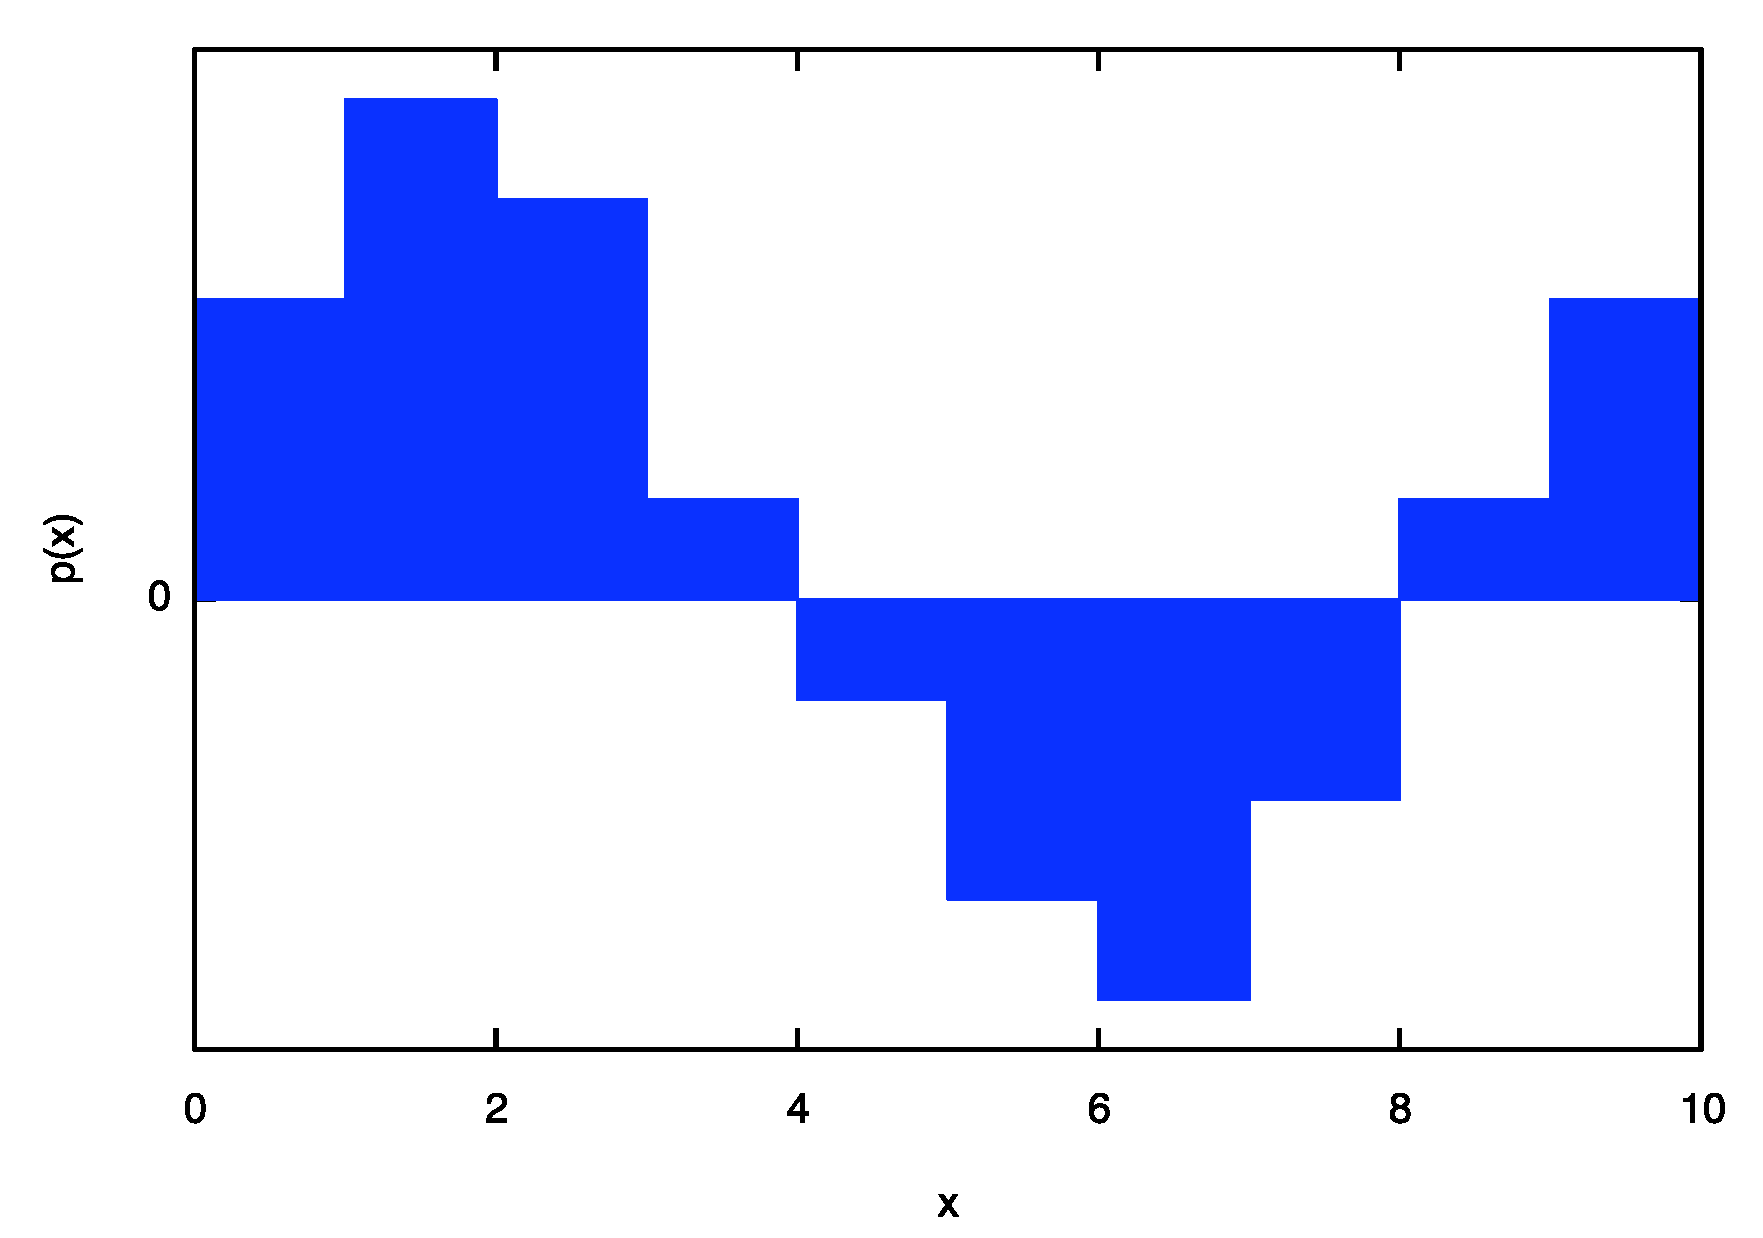
\includegraphics[width=\textwidth, keepaspectratio]{FullPDF}}
    \only<2>{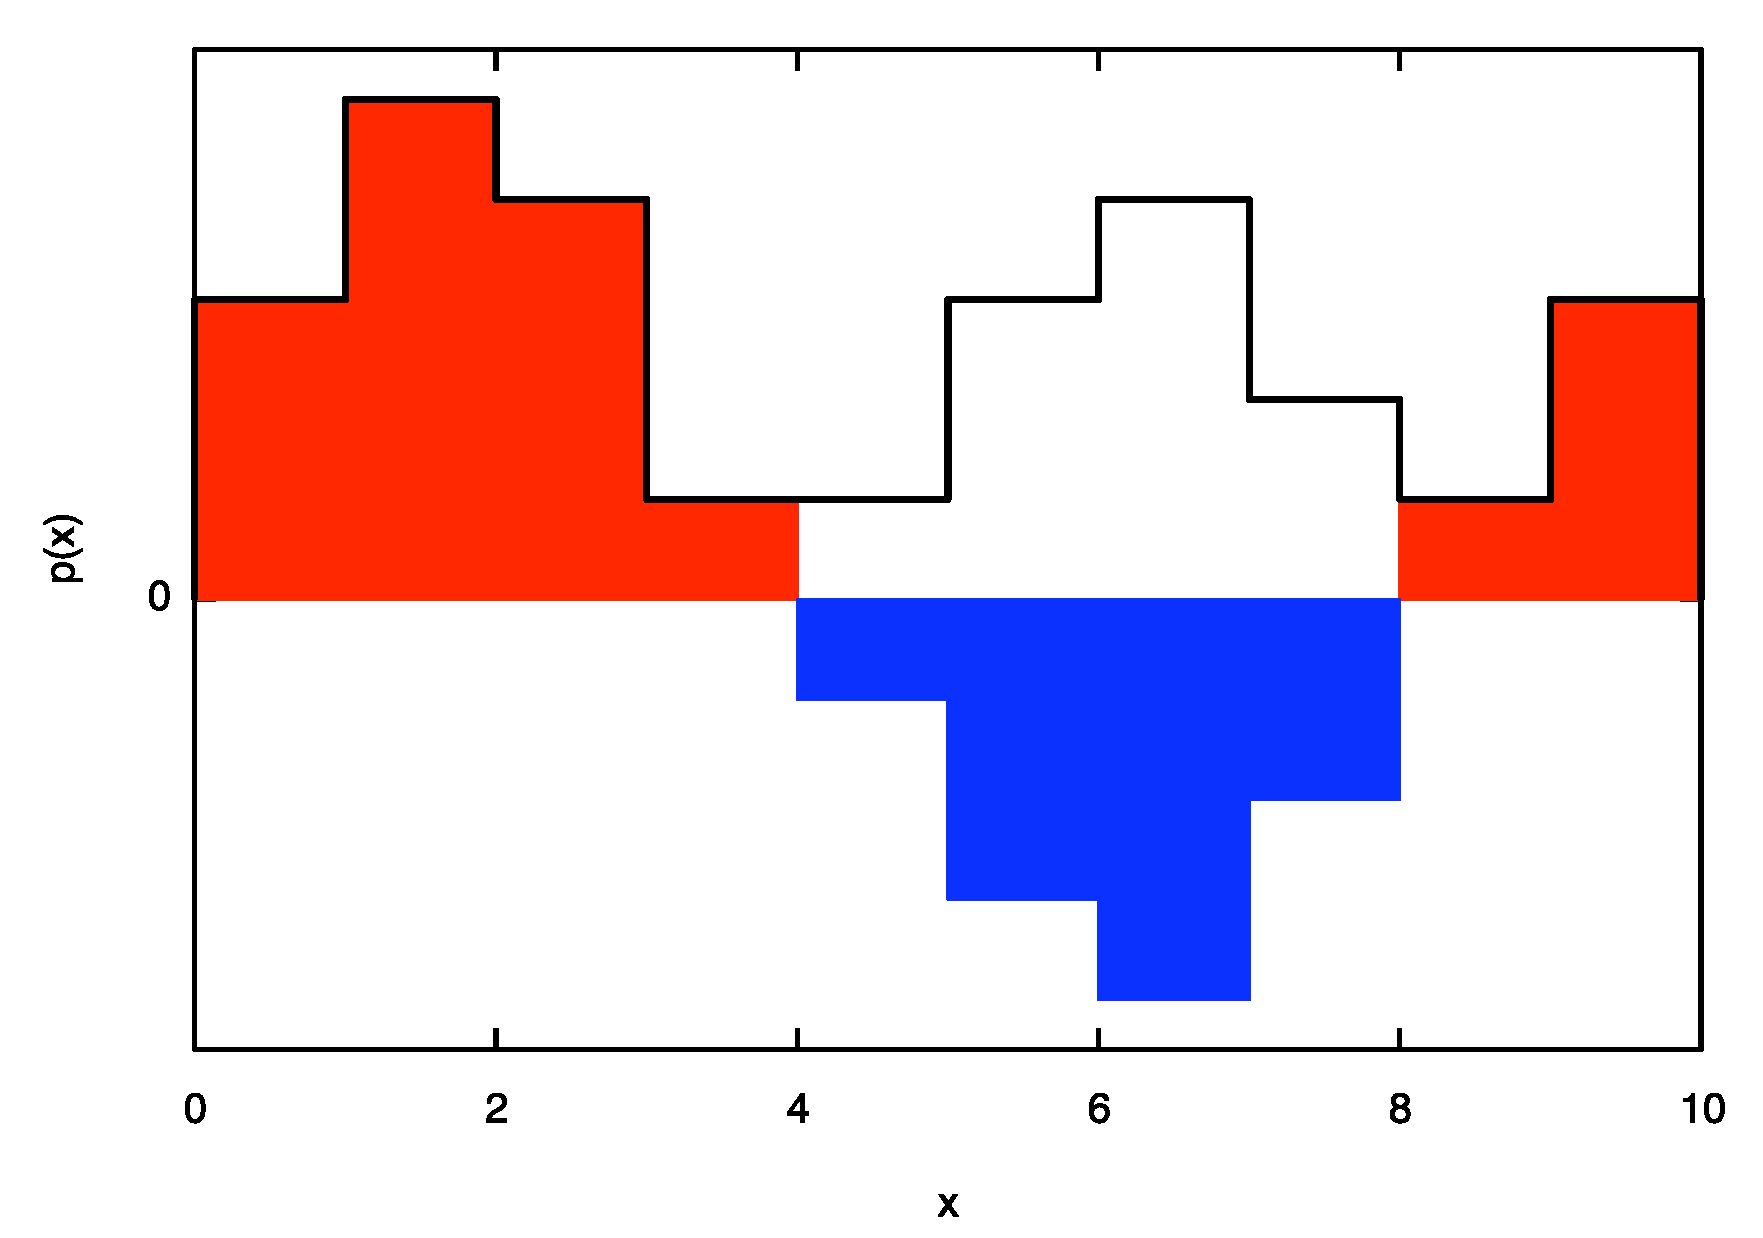
\includegraphics[width=\textwidth, keepaspectratio]{SplitPDF}}
%   \only<3>{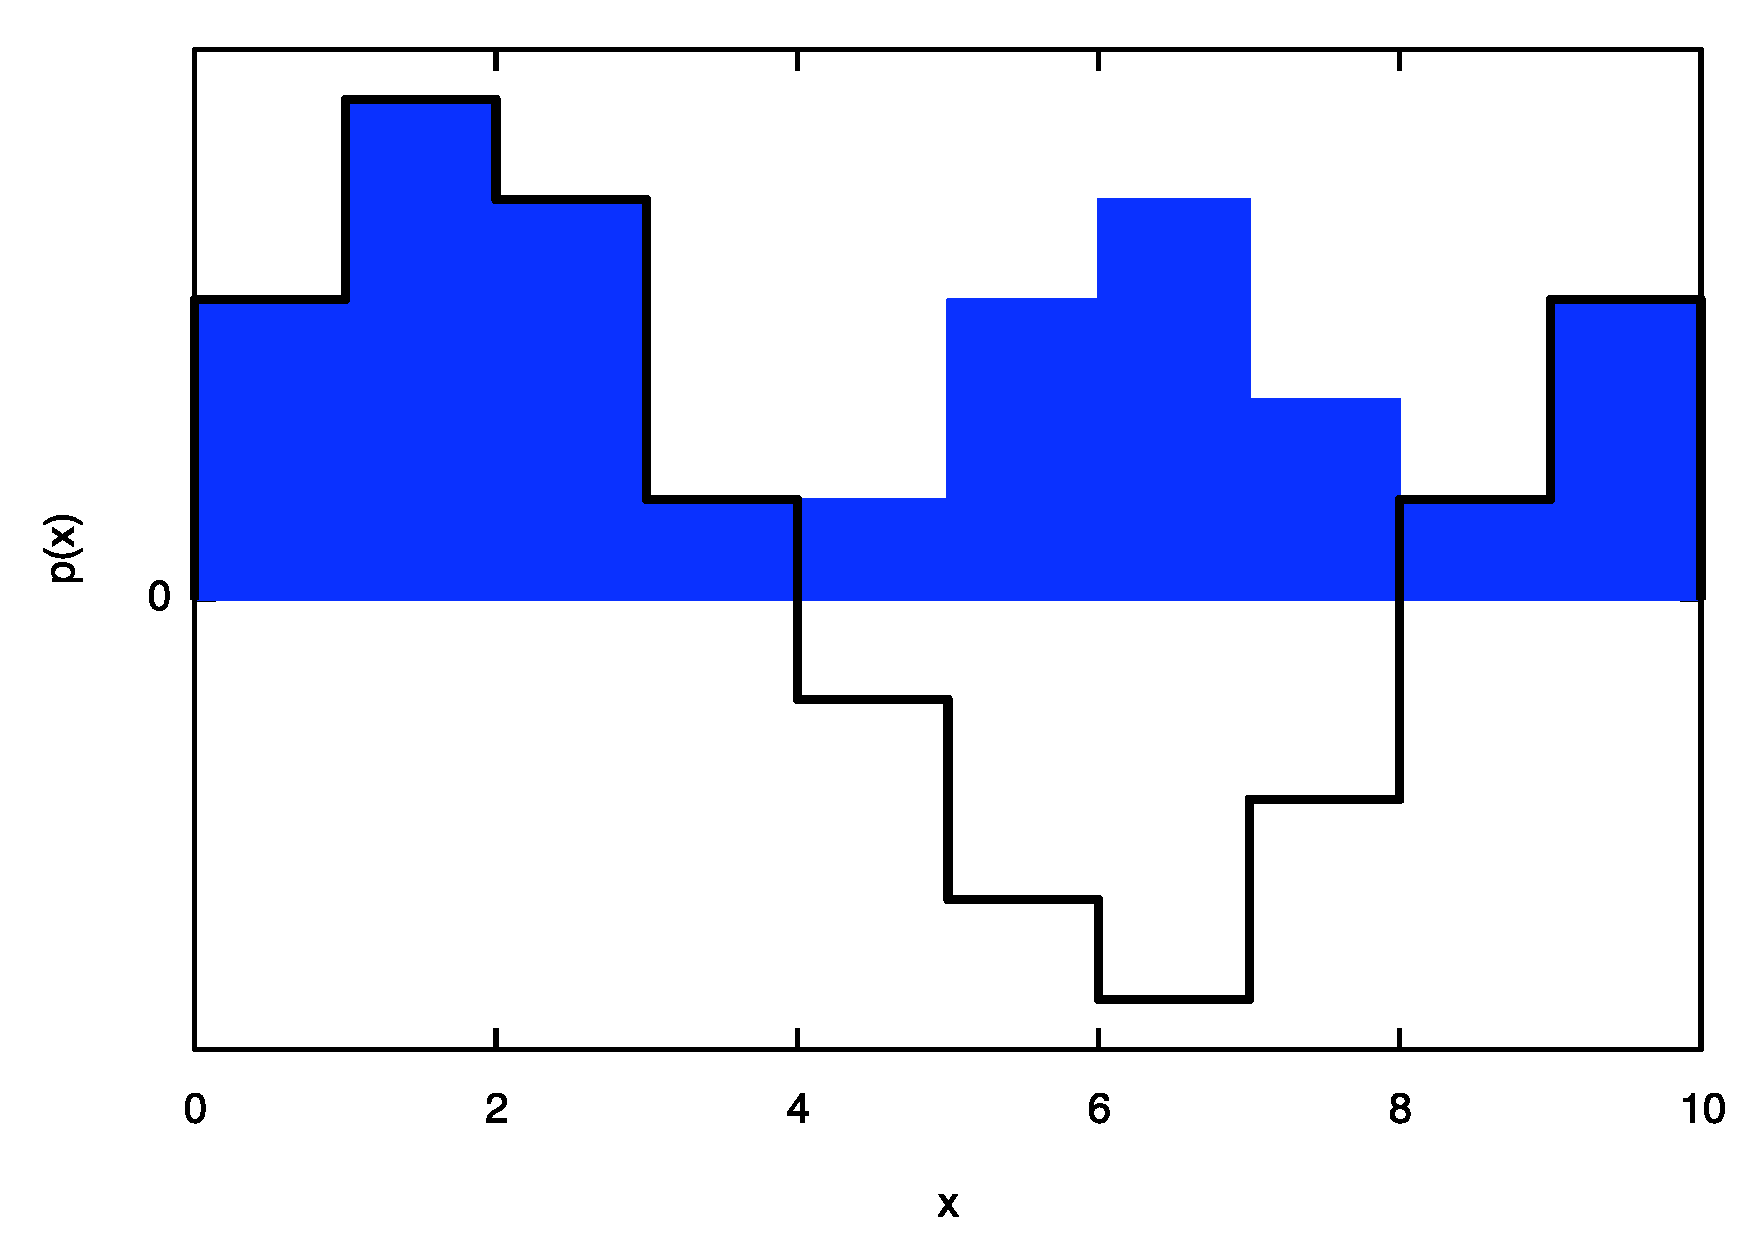
\includegraphics[width=\textwidth, keepaspectratio]{PosPDF}}
\end{frame}

\begin{frame}
    \frametitle{Negative Sources}
    \note{Through orthogonalization of Arnoldi vectors, some components of vectors will inevitably become negative}

    \begin{columns}[c]
    \column{0.5\textwidth}
        \begin{subequations}\begin{eqnarray*}
            \qp &=& \left\{
            \begin{array}{rc}
                q(x) ,& q(x) \geq 0 \\
                0 ,& \mathrm{else}
            \end{array}\right.  \\
            \qm &=& \left\{
            \begin{array}{rc}
                q(x) ,& q(x) < 0 \\
                0 ,& \mathrm{else}
            \end{array}\right. 
        \end{eqnarray*}\end{subequations}

    \column{0.5\textwidth}
        \only<1>{
        \begin{align*}
            q(x) &\equiv \qp + \qm \\[2ex]
            \A q(x) &= \A \qp - \A \qm
        \end{align*}
        }
        
        \only<2>{
        \begin{align*}
            p(x) &\equiv \frac{|q(x)|}{\int|q(x)|\,dx} \\
             &= \frac{\qp + |\qm|}{\int|q(x)|\,dx}
        \end{align*}
        }
    \end{columns}

    \note{Subtracting the negative source is equivalent to giving particles negative weight transporting and scoring as usual.}
\end{frame}

\section{Numerical Results}
\begin{frame}
    \frametitle{Problem Parameters}
    \begin{itemize}
        \item Homogeneous slab geometry
        \item $\Sigma_s = 0.5$, $\nu\Sigma_f = 0.5$, $\Sigma_t = 1.0$
        \item Both methods tracked the same number of particles
    \end{itemize}

%   \vspace{0.25in}
    \begin{table}[h]
        \centering
        \begin{tabular}{cccccc}
            \toprule
            Width & Spatial & \multirow{2}{10ex}{Particles} & \multirow{2}{10ex}{Iterations} & Inactive & Active \\
            (mfp) & Bins & & & Restarts & Restarts \\
            \midrule
            \multirow{2}{\LL}{20} & \multirow{2}{\LL}{75} & \multirow{2}{\LL}{500,000} & 20 & 2 & 20 \\
            & & & \multicolumn{3}{c}{40/400 power cycles} \\
            \midrule
            \multirow{2}{\LL}{50} & \multirow{2}{\LL}{75} & \multirow{2}{\LL}{500,000} & 30 & 10 & 30 \\
            & & & \multicolumn{3}{c}{300/900 power cycles} \\
            \midrule
            \multirow{2}{\LL}{100} & \multirow{2}{\LL}{100} & \multirow{2}{\LL}{10,000,000} & 30 & 5 & 25 \\
            & & & \multicolumn{3}{c}{150/750 power cycles} \\
            \bottomrule
        \end{tabular}
    \end{table}
\end{frame}

\begin{frame}
    \frametitle{Numerical Results}
\begin{table}[h]
    \centering
    \begin{tabular}{ccccc}
        \toprule
        Width (mfp) & $\lambda_0$ & Method & Eigenvalue &  Runtime (s) \\
        \midrule
        \multirow{2}{5mm}{20} & \multirow{2}{15mm}{0.985928} & Power & 0.98590 $\pm$ 0.00006 & 833 \\
                           & & Arnoldi & 0.9857 $\pm$ 0.0002 & 767 \\
        \midrule
        \multirow{2}{5mm}{50} & \multirow{2}{15mm}{0.99752} & Power & 0.99753 $\pm$ 0.00004 & 2307 \\
                           & & Arnoldi & 0.9976 $\pm$ 0.0002 & 2156 \\
       \midrule
       \multirow{2}{5mm}{100} & \multirow{2}{15mm}{0.99933} & Power & 0.99929 $\pm$ 0.00001 & 42820 \\
                          & & Arnoldi & 0.99926 $\pm$ 0.00007 & 35240 \\
        \bottomrule
    \end{tabular}
    \label{tab:results}
\end{table}

\vspace{2ex}
{\scriptsize Jeremy Lloyd Conlin and James Paul Holloway, \emph{Arnoldi's method of minimized iterations for Monte Carlo criticality calculations}, PHYSOR 2008, Interlaken, Switzerland}
\end{frame}

\begin{frame}
    \only<1>{\frametitle{Eigenvalue Convergence---20 mfp}
    \begin{center}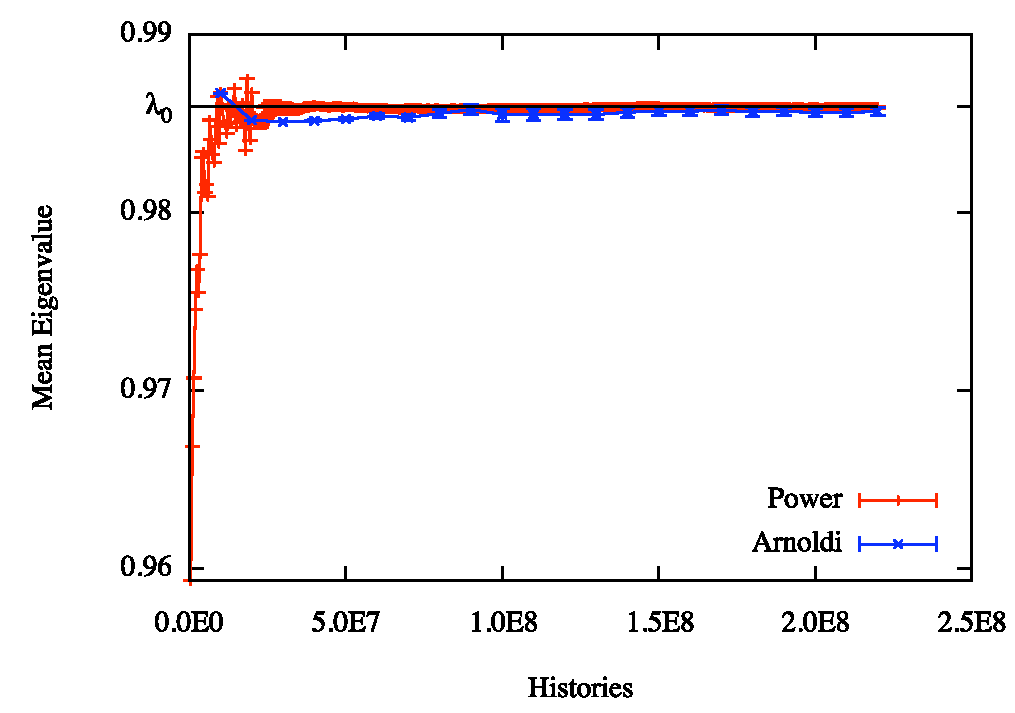
\includegraphics[width=0.90\textwidth, keepaspectratio]{ThinValue}\end{center}}
    \only<2>{\frametitle{Eigenvalue Convergence---50 mfp}
    \begin{center}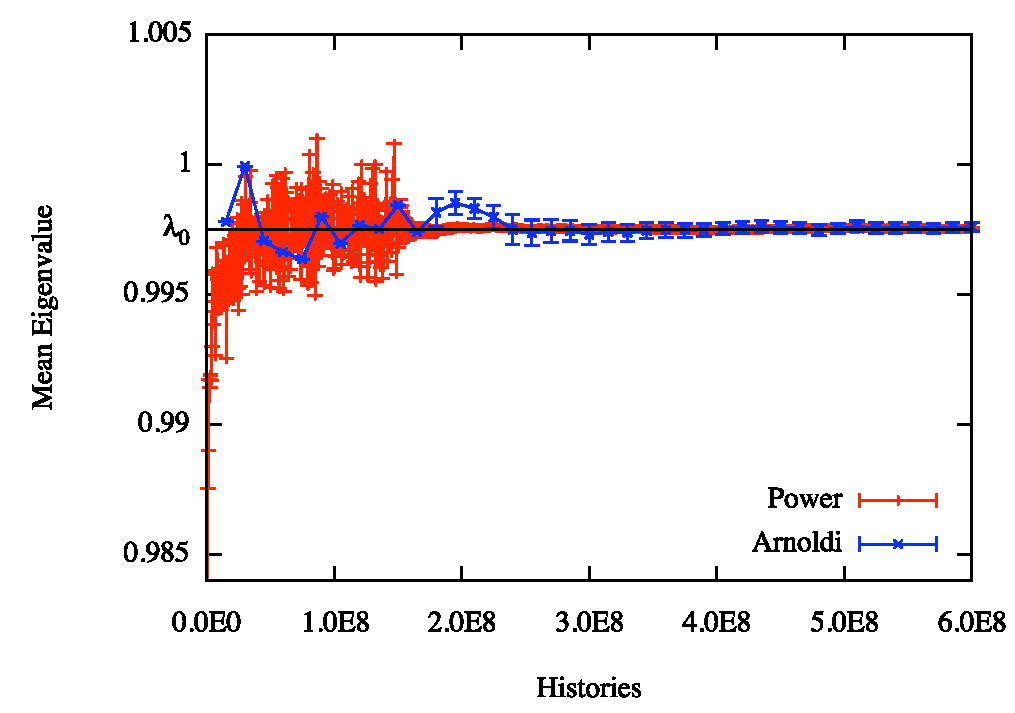
\includegraphics[width=0.90\textwidth, keepaspectratio]{MedValue}\end{center}}
    \only<3>{\frametitle{Eigenvalue Convergence---100 mfp}
    \begin{center}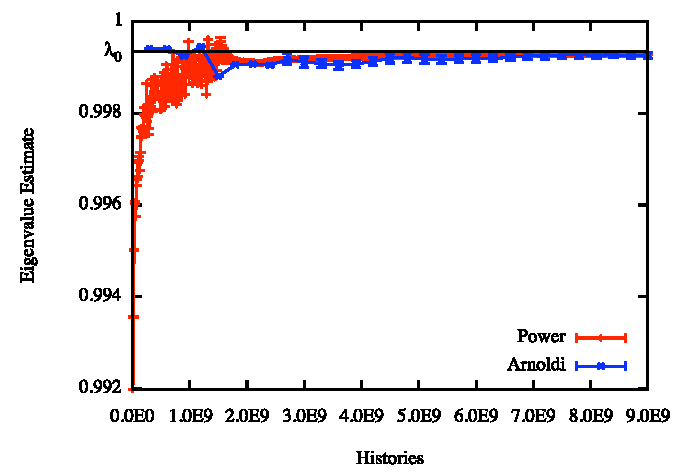
\includegraphics[width=0.90\textwidth, keepaspectratio]{ThickValue}\end{center}}
\end{frame}

\begin{frame}
    \frametitle{Eigenvectors}
    \only<1>{\begin{center}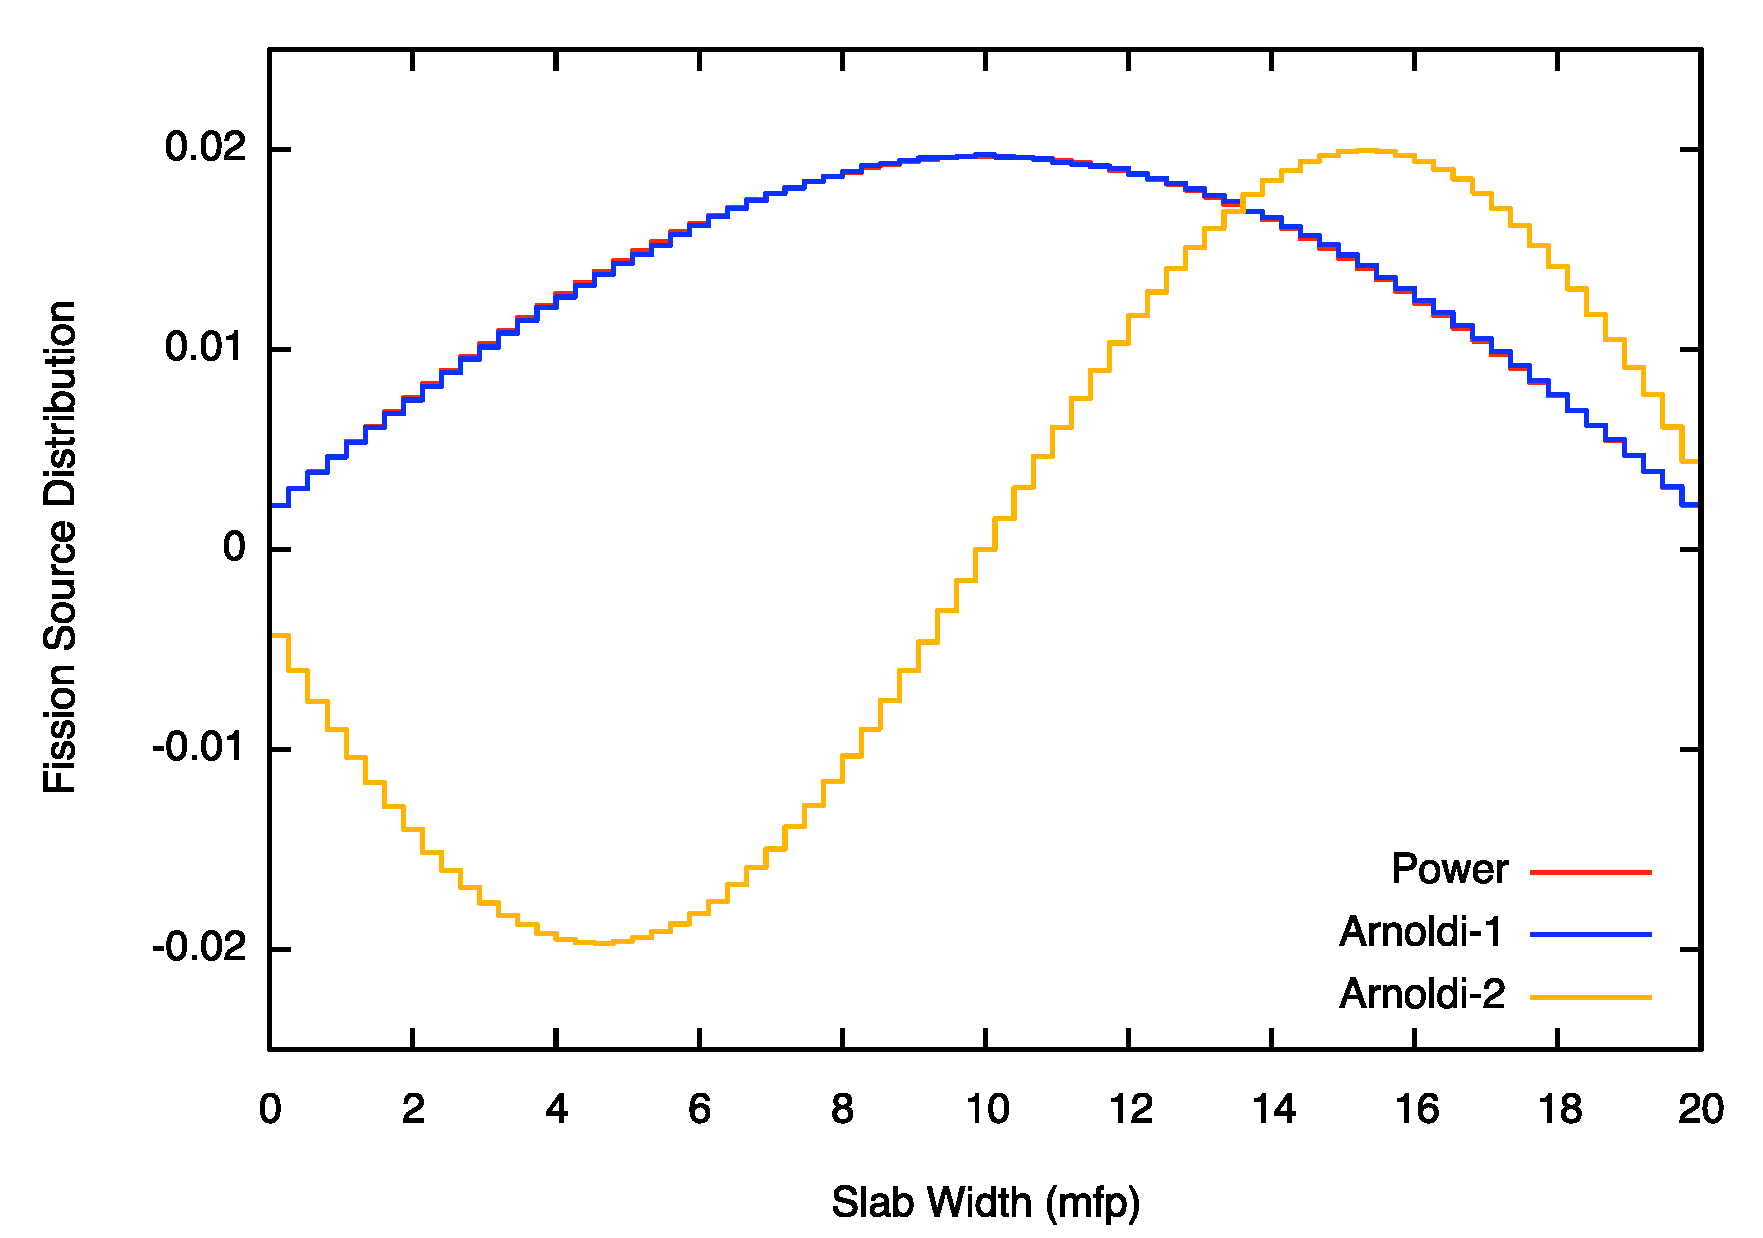
\includegraphics[width=0.90\textwidth, keepaspectratio]{ThinVector}\end{center}}
%   \only<2>{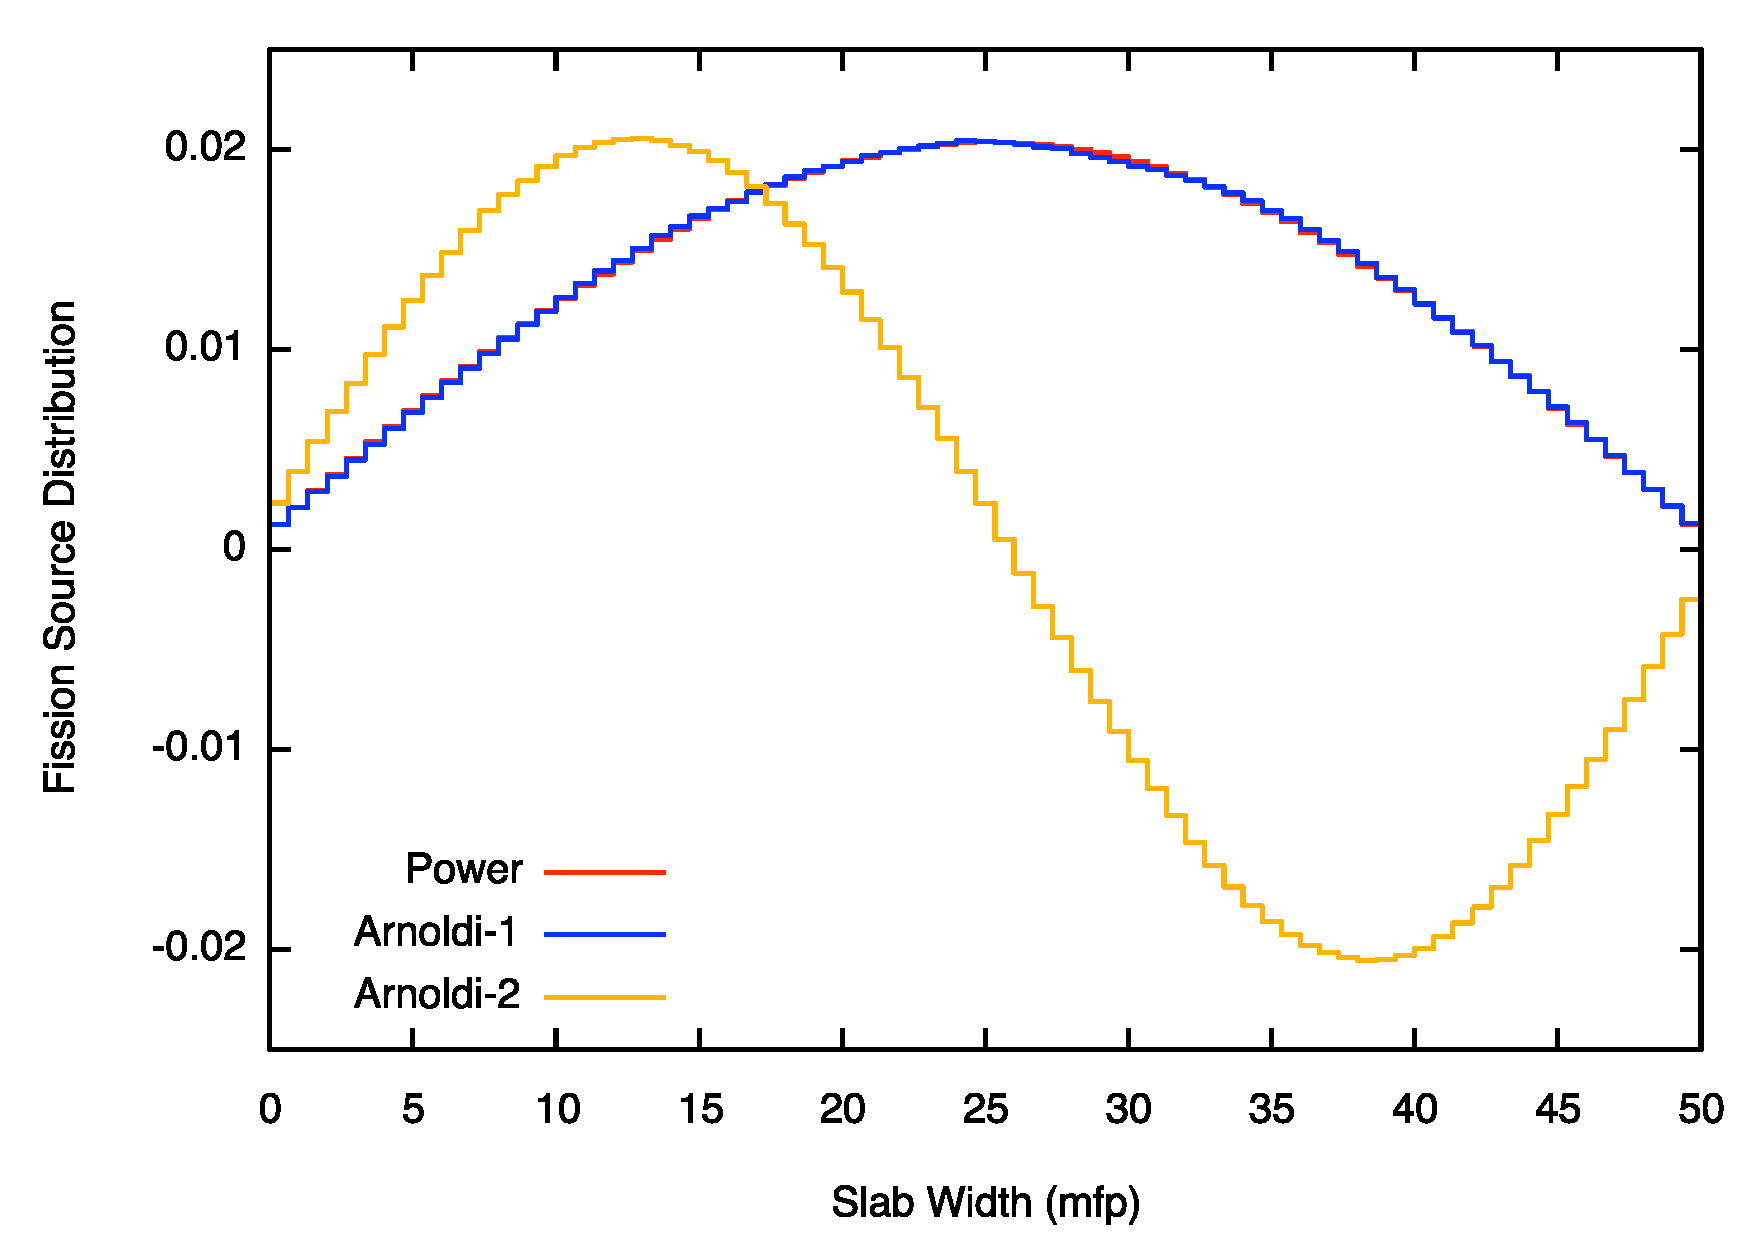
\includegraphics[width=\textwidth, keepaspectratio]{MedVector}}
%   \only<3>{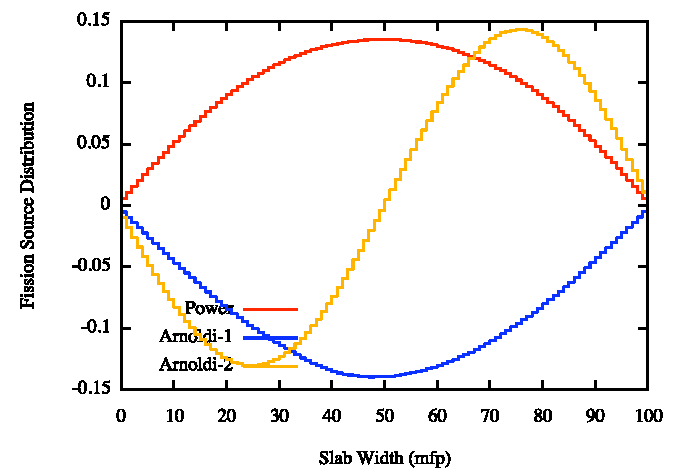
\includegraphics[width=\textwidth, keepaspectratio]{ThickVector}}
\end{frame}

\subsection{Discretization}
\begin{frame}
    \frametitle{Discretization Bias}
    \begin{center}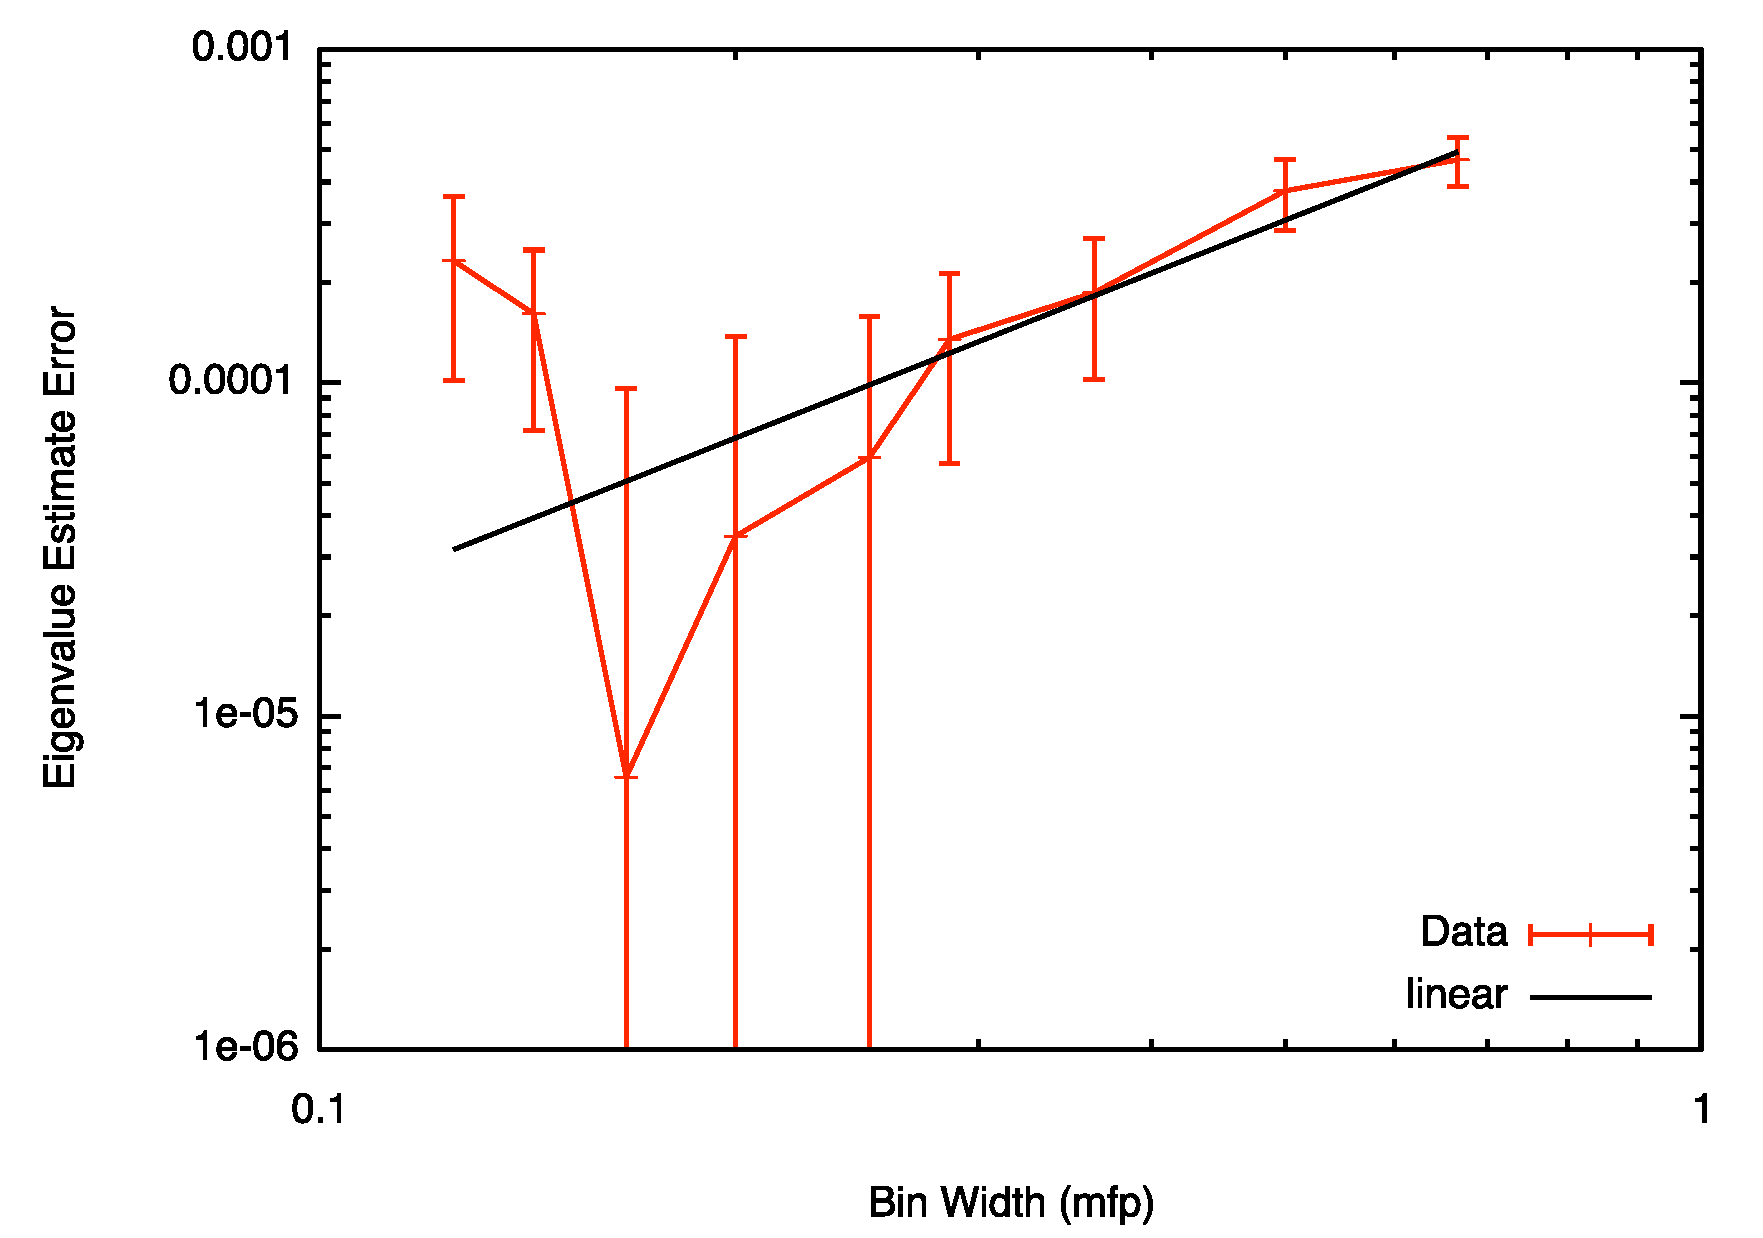
\includegraphics[width=0.90\textwidth, keepaspectratio]{Bias}\end{center}
\end{frame}

\subsection{Relaxed Matrix-vector Products}

\subsection{Relaxed Arnoldi's Method}
\begin{frame}
    \frametitle{Relaxed Arnoldi's Method}
    \begin{equation*}
        r_m = \left\|\A y_m - \lambda y_m\right\| = \left|q_{m+1}h_{m+1,m}e_m^Tx_m\right|
    \end{equation*}
    \note{We know that as the residual decreases, our estimate of the Ritz value becomes a better estimate of the eigenvalue of $\A$}
    \pause

    Bouras and Frayss\'{e}:
    \begin{itemize}
        \item Can \emph{relax} application of linear operator
        \item Maintain convergence of Arnoldi's method
        \item Save computational expense
    \end{itemize}
\end{frame}

\begin{frame}
    \frametitle{Relaxed Arnoldi's Method}
    \begin{equation*}
        \hat{q}_{m+1} = \left(\A + \DA\right)q_m
    \end{equation*}
    \pause

    Magnitude of $\DA$ is prevented from growing too large
    \begin{gather*}
        \alpha_k = \frac{1}{\min\left(\left\|r_{k-1}\right\|, 1\right)} \\[2mm]
        \left\|\DA_k\right\| = \varepsilon_k \left\|\A\right\|
    \end{gather*}
    where $\varepsilon_k = \min\left(\alpha_k \eta, 1\right)$.

    \vspace{2ex}
    \pause
    As residual decreases, precision of application of linear operator decreases.


\end{frame}

\begin{frame}
    \frametitle{Monte Carlo Relaxation}
    \begin{align*}
        \hat{q}_{m+1} &= \left(\A + \DA\right)q_m \\
        \DA &\propto \frac{1}{\sqrt{N}}
    \end{align*}
    More than 80\% of time spent on tracking particles (application of $\A$)

    \pause
    \vspace{2ex}
    How to relax Monte Carlo\pause---track fewer particles when residual is small
    \begin{equation*}
        N_k = \left \{ 
            \begin{array}{ccc}
                N_0 &, & \eta < r_{k-1} \\
                N_0 \left( r_{k-1}/\eta \right) &, & \eta \geq r_{k-1},
            \end{array}
            \right.
    \end{equation*}
\end{frame}

\begin{frame}
    \frametitle{Problem Parameters}
    \begin{itemize}
        \item Homogeneous slab geometry
        \item 20mfp thick
        \item 1E6 particles per iteration
        \item $\eta = 0.1$ for relaxed Arnoldi
    \end{itemize}

    \begin{table}[h]
        \centering
        \begin{tabular}{ccccc}
            \toprule
            \multirow{2}{10ex}{Material} & \multirow{2}{10ex}{Method} & \multirow{2}{10ex}{Iterations} & Inactive & Active \\
            & & & Restarts & Restarts \\
            \midrule
            \multirow{3}{10ex}{Absorbing} & Power & \multicolumn{3}{c}{50/280 power cycles} \\
            & Arnoldi & 10 & 5 & 28 \\
            & Relaxed Arnoldi & 10 & 5 & 150 \\
            \midrule
            \multirow{3}{10ex}{Scattering} & Power & \multicolumn{3}{c}{150/250 power cycles} \\
            & Arnoldi & 10 & 15 & 25\\
            & Relaxed Arnoldi & 10 & 15 & 150\\
            \bottomrule
        \end{tabular}
    \end{table}
\end{frame}

\begin{frame}
    \frametitle{Numerical Results}
\begin{table}
    \centering
    \begin{tabular}{cccc}
        \toprule
        Material & $\lambda_0$ & Method & Eigenvalue \\
        \midrule
        \multirow{3}{15mm}{Absorbing} & \multirow{3}{15mm}{0.98593} & Power & 0.98593 $\pm$ 0.00004 \\ % 20mfp.Power.short
        & & Arnoldi & 0.98590 $\pm$ 0.00008 \\ % 20mfp.NotRelaxed4
        & & Relaxed Arnoldi & 0.98592 $\pm$ 0.00006 \\ % 20mfpRelaxed
        \midrule
        \multirow{3}{15mm}{Scattering} & \multirow{3}{15mm}{0.93339} & Power & 0.93335 $\pm$ 0.00008 \\ % 20mfp.Scattering.NotRelaxed.i15.Power.dat active: 250
        & & Arnoldi & 0.93331 $\pm$ 0.00023 \\ % 20mfp.Scattering.NotRelaxed.i15.dat Restart #: 24
        & & Relaxed Arnoldi & 0.93338 $\pm$ 0.00008 \\ % 20mfp.Scattering.x0.1.i15.Long.dat
        \bottomrule
    \end{tabular}
\end{table}

    \vspace{2ex}
    {\scriptsize Jeremy Lloyd Conlin and James Paul Holloway, \emph{Relaxation scheme for Monte Carlo explicitly restarted Arnoldi's method for criticality calculations}, M\&C 2009, Saratoga Springs, NY}
\end{frame}

\begin{frame}
    \only<1>{\frametitle{Eigenvalue Convergence---Absorbing Material}
    \begin{center}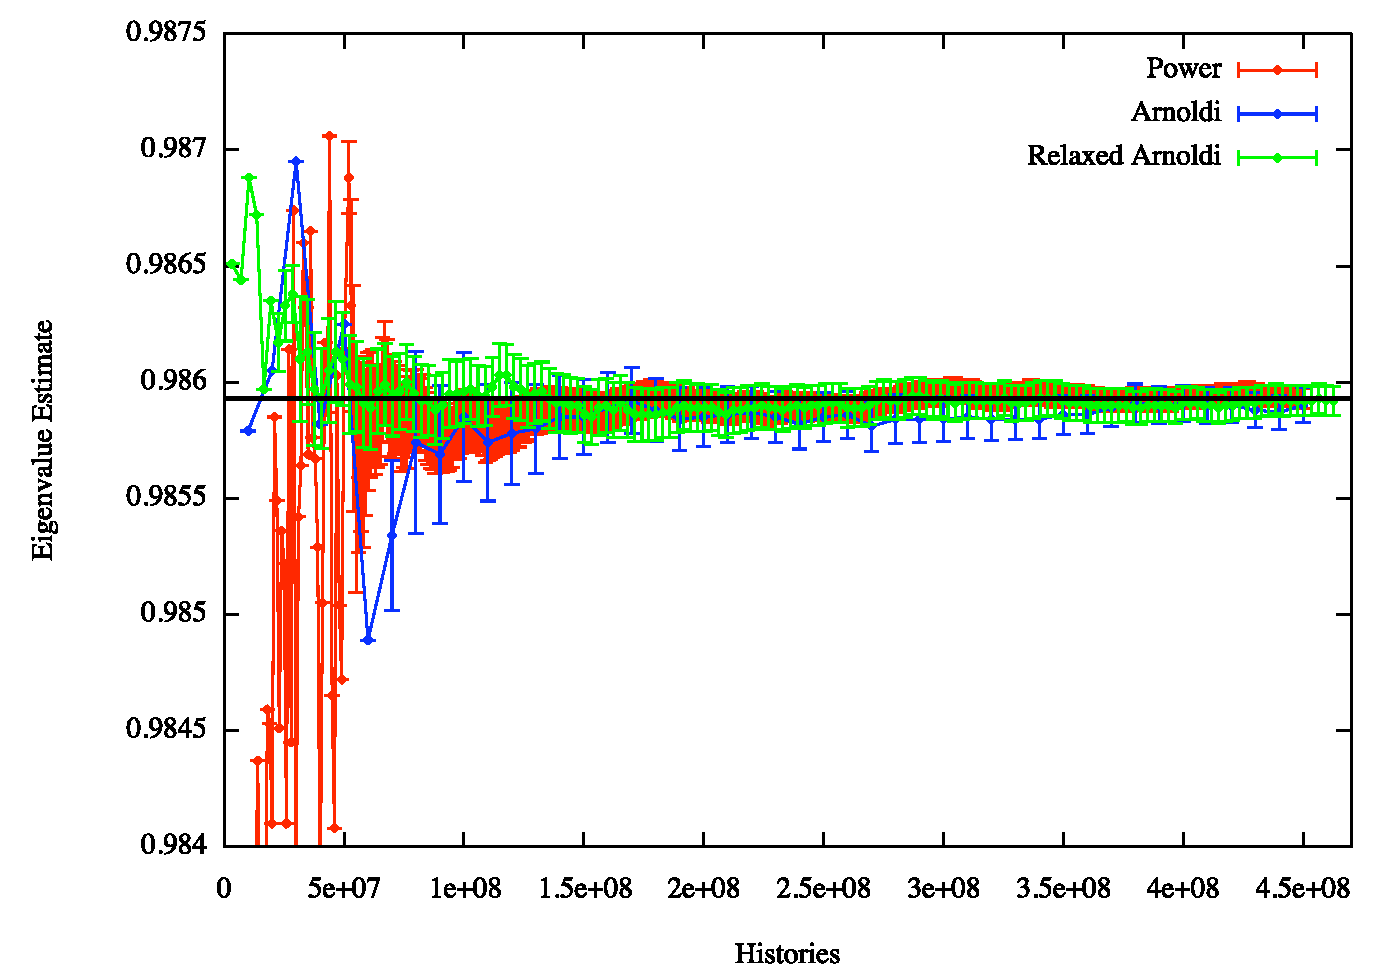
\includegraphics[width=0.9\textwidth,keepaspectratio]{ValueAbsorbing} \end{center}}
    \only<2>{\frametitle{Eigenvalue Convergence---Scattering Material}
    \begin{center}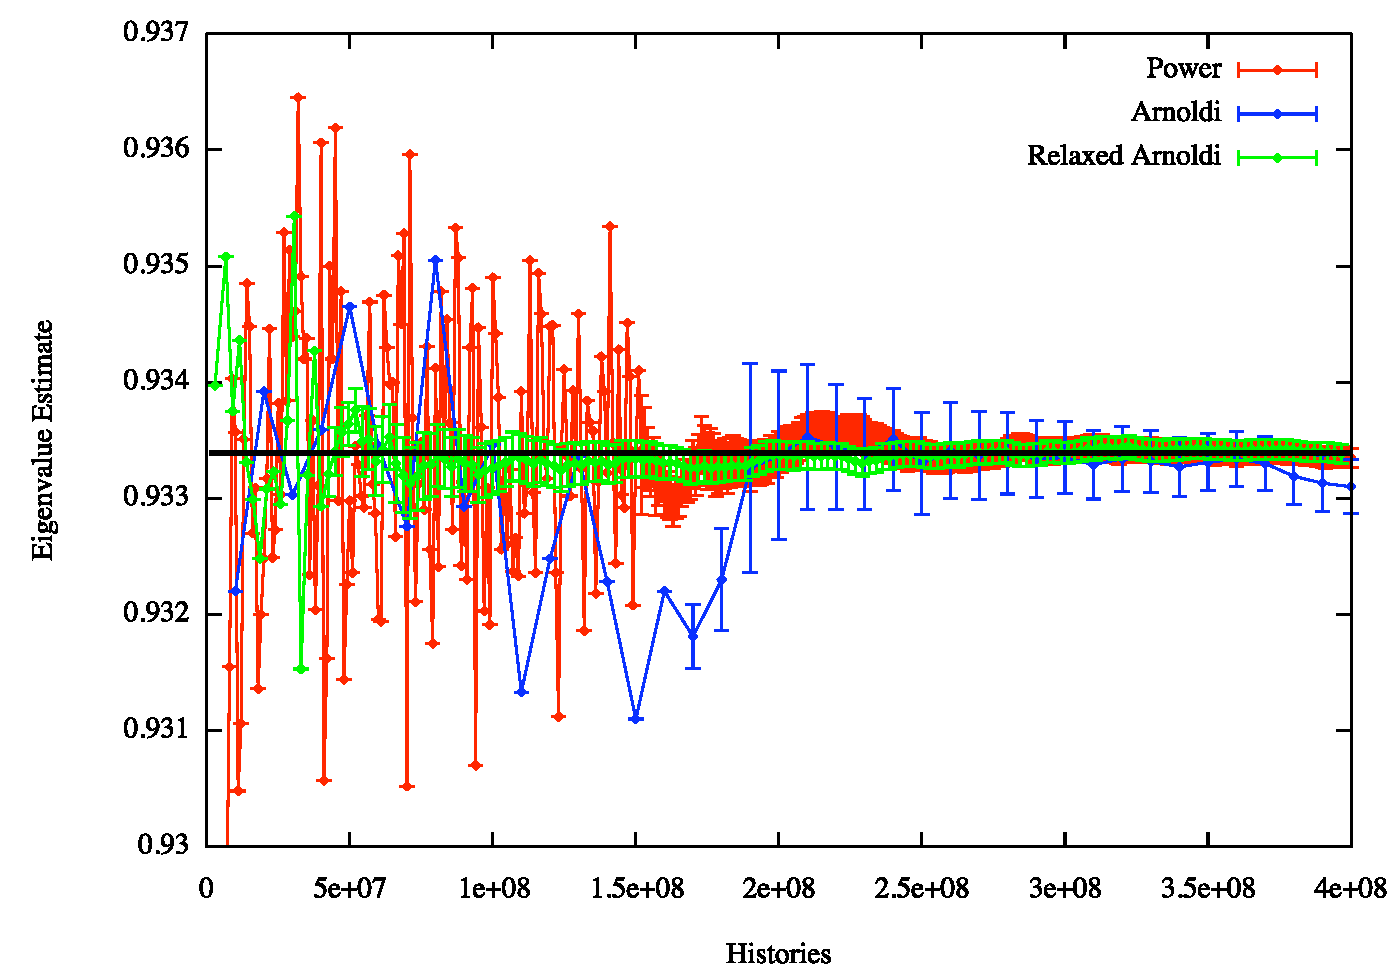
\includegraphics[width=0.9\textwidth,keepaspectratio]{ValueScattering} \end{center}}
\end{frame}

\begin{frame}
    \frametitle{Relaxed Timing Results}
    \begin{table}
        \centering
        \begin{tabular}{cccccc}
            \toprule
            Material & Method & Runtime (s) & Particles/sec & Cost \\
            \midrule
            \multirow{3}{15mm}{Absorbing} & Power & 1742 & $2.58 \times 10^5$  & 1 \\ % 20mfp.Power.short
            & Arnoldi & 1669 & $2.70 \times 10^5$ & 0.956 \\ % 20mfp.NotRelaxed4
            & Relaxed Arnoldi & 1972 & $2.34 \times 10^5$ & 1.100 \\ % 20mfpRelaxed
            \midrule
            \multirow{3}{15mm}{Scattering} & Power & 2310 & $1.73 \times 10^5$  & 1 \\ % 20mfp.Scattering.NotRelaxed.i15.Power.dat active:250
            & Arnoldi & 2340 & $1.71 \times 10^5$ & 1.01 \\ % 20mfp.Scattering.NotRelaxed.i15.dat Restart #: 24
            & Relaxed Arnoldi & 2272 & $1.75 \times 10^5$ & 0.989 \\ % 20mfp.Scattering.x0.1.i15.Long.dat
            \bottomrule
        \end{tabular}
        \label{tab:Timing}
    \end{table}
\end{frame}

\begin{frame}
    \only<1>{\frametitle{Uncertainty---Absorbing Material}
    \begin{center}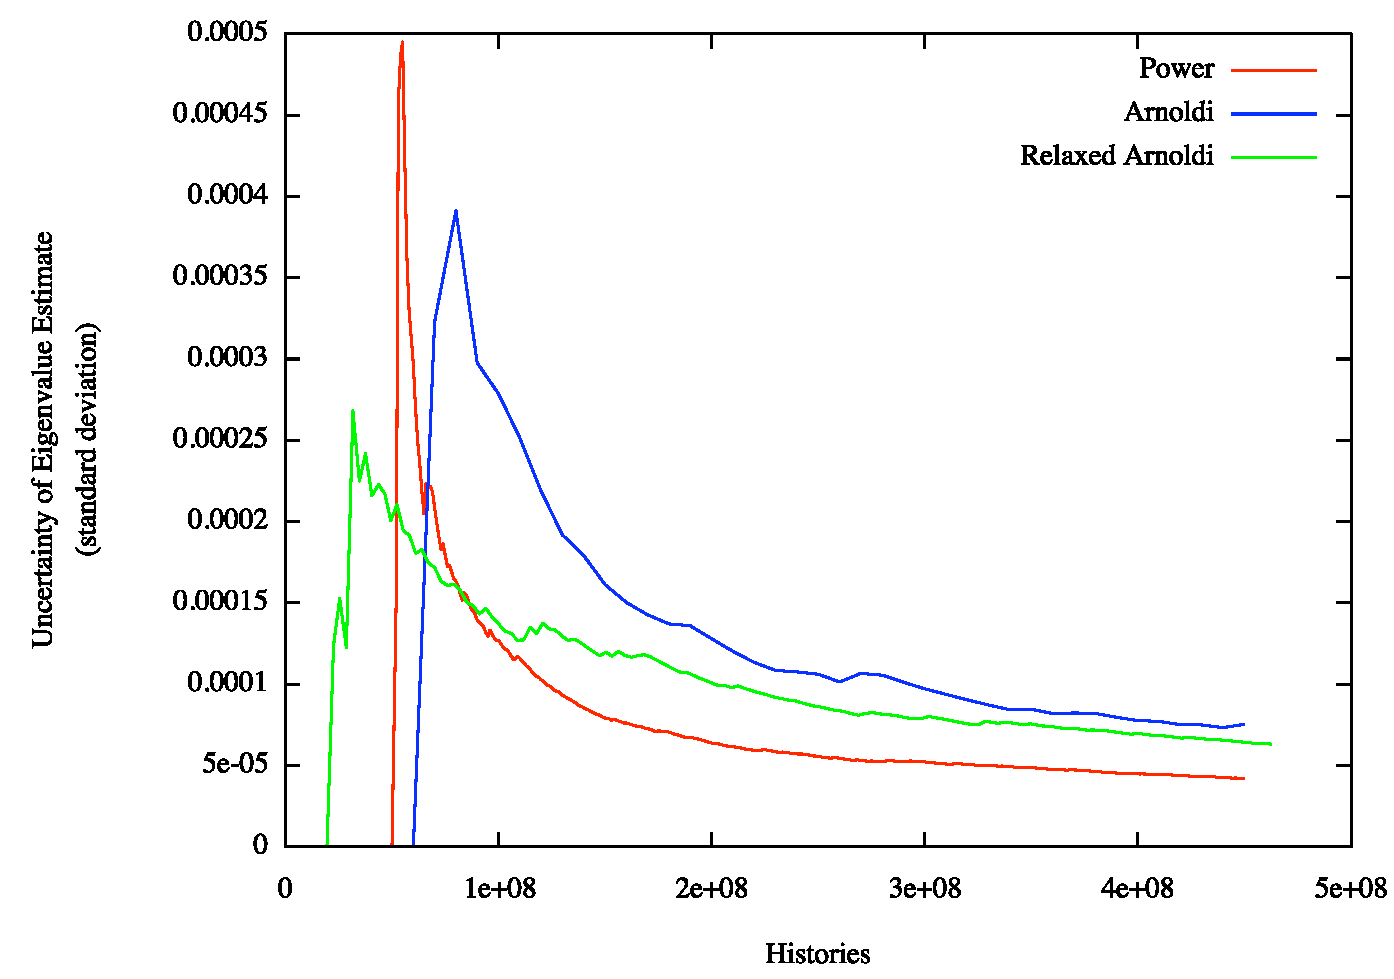
\includegraphics[width=0.9\textwidth,keepaspectratio]{UncertaintyAbsorbing} \end{center}}
%   \begin{center}\includegraphics[width=0.9\textwidth,keepaspectratio]{UncertaintyAbsorbingLogLog}\end{center}}
    \only<2>{\frametitle{Uncertainty---Scattering Material}
    \begin{center}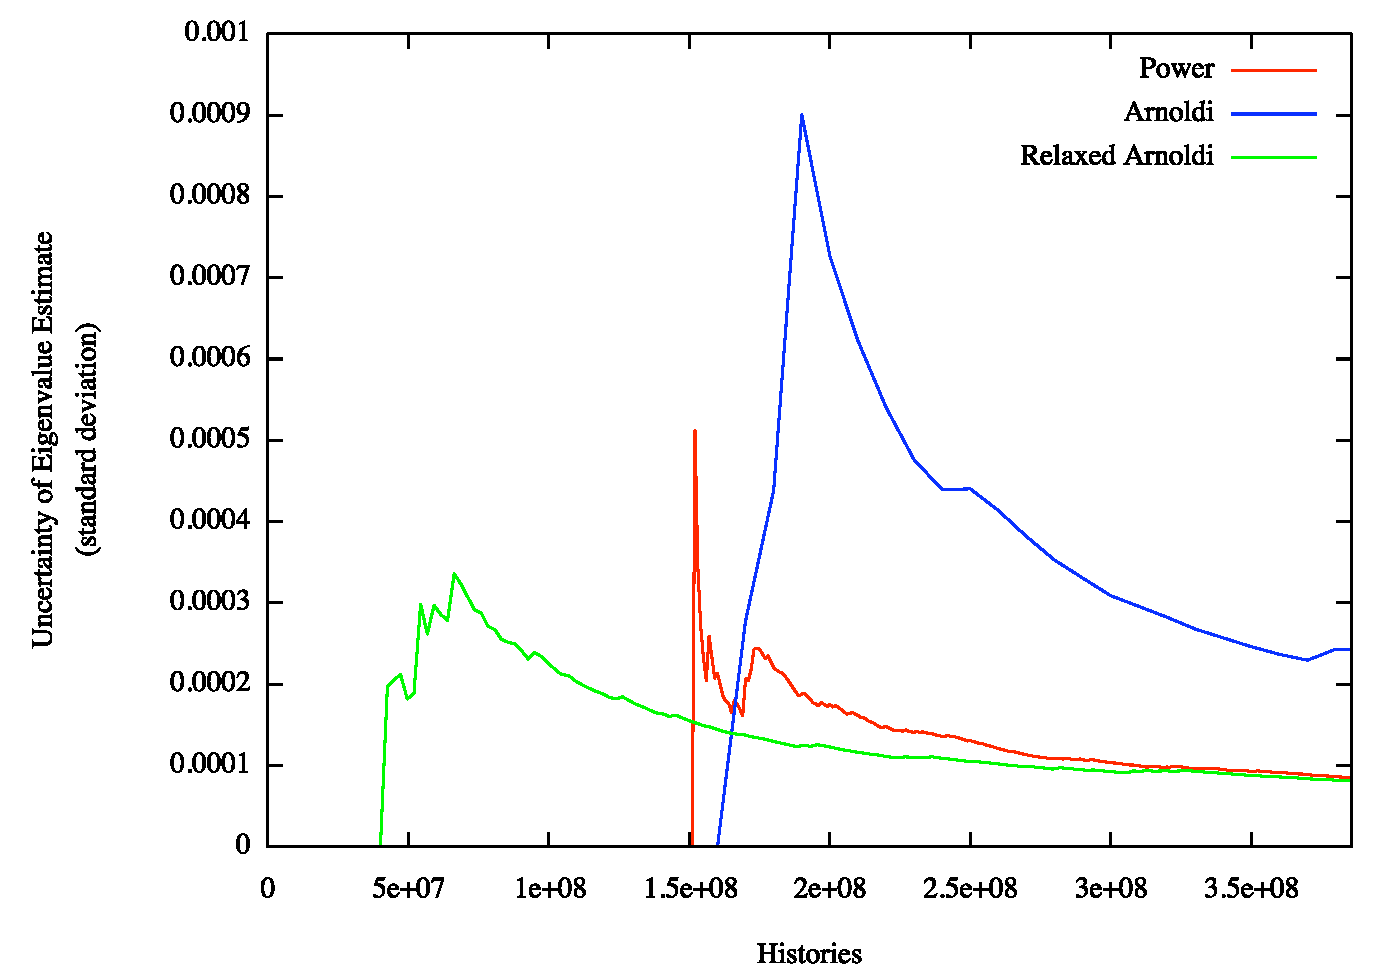
\includegraphics[width=0.9\textwidth,keepaspectratio]{UncertaintyScattering} \end{center}}
%   \begin{center}\includegraphics[width=0.9\textwidth,keepaspectratio]{UncertaintyScatteringLogLog}\end{center}}
\end{frame}


\subsection{Discussion}
\begin{frame}
    \frametitle{Discussion}
    Arnoldi's method:
    \begin{itemize}
        \item Can be used in Monte Carlo criticality applications
        \item Can calculate higher order eigenmodes
        \item Should be relaxed to reduce uncertainty and possibly save time
    \end{itemize}
\end{frame}

\section{Future Work}
\subsection{Implicitly Restarted Arnoldi's Method}
\begin{frame}
    \frametitle{Outline}
    \tableofcontents[pausesection]
\end{frame}

\begin{frame}
    \frametitle{Restarted Arnoldi}
    \begin{equation*}
        \A Q_m = Q_{m}H_{m} + r_m
    \end{equation*}
    \vspace{2ex}
    Restart vector:
    \begin{equation*}
        q_0 = a_0y_0 + a_1y_1 + \cdots + a_{n-1}y_{n-1}
    \end{equation*}
    
    \pause
    \begin{itemize}[<+->]
        \item Desire $j$ eigenpairs
        \item Want $a_j, \cdots, a_{n-1}$ to be small
        \item Explicit restarts force $a_j = \cdots = a_{n-1} = 0$
    \end{itemize}
\end{frame}

\begin{frame}
    \frametitle{Implicit Restarts}
    Replace Arnoldi Iterations with shifted QR-algorithm iterations on $H_m$
    \begin{gather*}
       \left(H_m - \mu_1I\right) = V_1R_1 \\[1ex]
       \hat{H}_1 = V_1^*H_mV_1
    \end{gather*}
    After $j$ iterations
    \begin{equation*}
        \hat{H}_p = \hat{V}_p^*H_m\hat{V}_p
    \end{equation*}
    where 
    \begin{equation*}
        \hat{V}_p = V_1V_2\cdots V_p
    \end{equation*}
\end{frame}

\begin{frame}
    \frametitle{Implicit Restarts}
    Substitute $H_m = \hat{V}_pH_m\hat{V}_p^*$ into Arnoldi factorization

    \begin{align*}
        \A Q_m &= Q_{m}H_{m} + r_m \\
        \A Q_m &= Q_{m}\hat{V}_pH_m\hat{V}_p^* + r_m \\
        \A Q_m\hat{V}_p &= Q_{m}\hat{V}_pH_m\hat{V}_p^*\hat{V}_p + r_m\hat{V}_p \\
        \A \hat{Q}_m &= \hat{Q}_mH_m + r_m\hat{V}_p
    \end{align*}
    where $\hat{Q}_m = Q_m\hat{V}_p$.

\end{frame}

\begin{frame}
    \frametitle{Implicit Restarts}
    \begin{equation*}
        \A \hat{Q}_m = \hat{Q}_mH_m + r_m\hat{V}_p
    \end{equation*}

    \begin{itemize}
        \item Arnoldi factorization
        \item Restarted with $p$ iterations of shifted QR-algorithm
        \pause
        \item If shifts are chosen judiciously:
            \begin{itemize}
                \item Implicit restart equivalent to explicit restart
                \item Suppresses unwanted portion of spectrum of $\A$
                \item Implicit restarts can then proceed at iteration $p+1$
            \end{itemize}
        \pause
        \item Implicit restarts trade applications of $\A$ for shifted QR-algorithm iterations
    \end{itemize}

    \note{$\A \hat{Q}_m &= \hat{Q}_pH_m + r_m\hat{V}_p$ is an Arnoldi factorization.  It can be shown that performing the shifted QR-algorithm iterations will produce a restart vector with the unwanted portion of the spectrum suppressed and starting with }
\end{frame}

\begin{frame}
    \frametitle{Questions}
\end{frame}

\end{document}
